\section{Thermal mass estimation}
\label{ch:thermtool}
Decelerating an entry vehicle requires a thermal protection system. This system will contribute to a large extend to the mass of the entire vehicle. Therefore, a \acrfull{tps} has a critical impact on the mission and should be selected properly. This section will analyse the \gls{tps} of the five trade-off concepts with the use of a thermal protection tool. Note that for the rigid concept a mass estimate is already given in \ref{sec:rigid} as the \gls{tps} is normally integrated in the structure. First the tool will be described in more detail. Afterwards it is described how the tool could not be verified and validated. In the third section, analysis of the different lay-ups for the concepts is done using a more simple approach since the tool does not function correctly. As a result, the relative \gls{tps}-masses for different concepts can be given. Lastly, the conclusions of this analysis and recommendations for future work are discussed.

\subsection{Method of thermal analysis}
A mass estimation of the \gls{tps} requires analysis due to heat transfer into the heat shield. Enabling the analysis of different lay-ups in a short amount of time, it will be useful to make use of a \gls{tps} tool. In this section the working principles of this is explained.

\subsubsection{Assumptions}
In this section the assumptions used for the \gls{tps} mass estimation and for the tool development are stated. Also, an elaboration is given on the impact of the assumptions on the results.

\begin{itemize}
\item \textbf{1D instead of 3D analysis}: For the determination of the temperature through the material over time, a one dimensional lay-up can be used. This is different from the actual case, where the body is heated over a three dimensional body. This assumption is verified for instance by Ref. \cite{Corso2009}.
\item \textbf{Sizing is done under stagnation conditions}: One of the inputs in the tool is the temperature at the wall. For this, the stagnation temperature is used instead of the actual temperature distribution over the surface. The stagnation temperature is a maximum value for the temperature and hence, the result of the tool will give the most conservative value needed for the design of the \gls{tps}. Therefore, the \gls{tps} will be over-designed and do not necessarily have to be used as final values of the \gls{tps} mass. However, they do give an indication on how different concepts perform relative to each other, such that the method can be used to make trade-off decisions.
\item \textbf{Model for heat flux}: Another input in the tool is the heat flux. This heat flux input is based on an aerodynamic model, as described in section\ref{subsec:aerotool}. As is explained there, the wall temperature ($\gls{sym:T}_w$) an omitted from the calculation. The tension cone and stacked toroid have the same shape in the aerodynamic tool, therefore the resulting heat flux is the same for both concepts.
\item \textbf{Constant material properties}: Material properties like tensile strength, density and thermal conductivity change, if considered over a large temperature range. However, it is assumed that this change is negligible for this low fidelity tool. 
\item \textbf{Use of ablative materials}: Ablative materials of rigid structures are assumed not to reduce in thickness as a first approximation.
\item \textbf{Applicable to multiple layers}: The tool uses steps in length that pass over layers with different materials. It is possible that a length step is located in between two layers but is only considered as one material. Because length steps are very small, this has no major impact on the model.
\item \textbf{Discretisation of differential equations}: The tool is based on a finite difference discretisation. This method is verified. However, the discretisation errors are only stable for a certain range of time steps, as can be seen in Ref. \cite{Smith2011,Holman2002}. 
\end{itemize}

\subsubsection{Leading equations}
The problem is modelled as a one-dimensional multilayer lay-up which can provide the accuracy needed for this stage of concept analysis as described in the assumptions. A description of the implementation of this model is given by Smith \cite{Smith2011}. The model is illustrated in Figure \ref{fig:1dthermal}. The figure shows the different methods of heat transfer in the model. There is heat radiating away from the surface, convective heating or heat flux from the aerodynamic effects and heat conduction within the layers.

\begin{figure}[H]
	\centering
	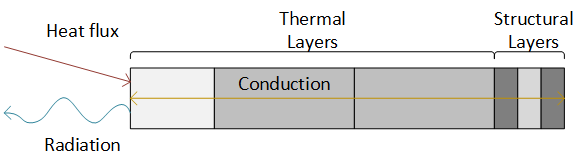
\includegraphics{Figure/1dthermal.png}
	\caption{1D thermal model}
	\label{fig:1dthermal}
\end{figure}

The layup is then discretised in $i_{max}$ nodes, each having a thickness of $\Delta \gls{sym:x}$. For the nodes that only experience conduction as heat transfer the one-dimensional, time-dependent (transient) heat equation can be used, which is given by Equation \eqref{eq:therm1}

\begin{equation}
\frac{\partial \gls{sym:T}}{\partial \gls{sym:t}} = \gls{sym:alphat}\frac{\partial^2\gls{sym:T}}{\partial \gls{sym:x}^2}
\label{eq:therm1}
\end{equation}

In this equation $\gls{sym:alphat}=\frac{\gls{sym:k}}{\rho \gls{sym:cp}}$ stands for the thermal diffusivity, \gls{sym:k} for the thermal conductivity, $\rho$ the material density and \gls{sym:cp} the material specific heat. Since the layup has been discretised, the heat equation is discretised as well. The time march method used for this discretisation is the Forward in Time and Central in Space (FTCS) scheme is used. The advantage of this time march is that it is computationally inexpensive. The drawback is that it can be unstable and therefore $\Delta \gls{sym:t}$ and $\Delta \gls{sym:x}$ should be chosen such that it complies with a stability criterion. The result of the time march is given by Equation \eqref{eq:therm2}. The notation in the equation is as follows: the subscript $i$ refers to the node and the superscript $n$ refers to the timestep. Obviously, the distance between $i$ and $i+1$ is $\Delta \gls{sym:x}$ and the time between $n$ and $n+1$ is $\Delta \gls{sym:t}$.

\begin{equation}
\frac{\gls{sym:T}_i^{n+1}-\gls{sym:T}_i^n}{\Delta \gls{sym:t}} = \gls{sym:alphat}\left[\frac{\gls{sym:T}_{i+1}^n-2\gls{sym:T}_i^n+\gls{sym:T}_{i-1}^n}{\left(\Delta \gls{sym:x}\right)^2}\right]
\label{eq:therm2}
\end{equation}

This equation can be rewritten such that it shows the heat rate balance of a node per unit area in $\left[\frac{W}{m^2}\right]$ (Equation \eqref{eq:therm3}). This can be done by writing out \gls{sym:alphat}. To account for different materials in the layup, the heat transfer between the neighbouring nodes is separated. For this the factors $\gls{sym:K}_{i-1}=2\left(\frac{1}{\gls{sym:k}_{i-1}}+\frac{1}{\gls{sym:k}_i}\right)^{-1}$ and $\gls{sym:K}_{i+1}=2\left(\frac{1}{\gls{sym:k}_{i+1}}+\frac{1}{\gls{sym:k}_i}\right)^{-1}$ are used. The same behaviour can be seen in electrical resistance as the inverse of the equivalent resistance is the sum of the inverse resistances in a parallel circuit ($\frac{1}{R_{eq}}=\frac{1}{R_1}+\frac{1}{R_2}$). This heat rate balance can also be presented schematically as shown in Figure \ref{fig:thermbalance1}.

\begin{equation}
\frac{\rho_i\gls{sym:cp}_i\Delta \gls{sym:x}}{\Delta \gls{sym:t}}\left(\gls{sym:T}_i^{n+1}-\gls{sym:T}_i^n\right)=\frac{\gls{sym:K}_{i-1}}{\Delta \gls{sym:x}}\left(\gls{sym:T}_{i-1}^n-\gls{sym:T}_i^n\right)-\frac{\gls{sym:K}_{i+1}}{\Delta \gls{sym:x}}\left(\gls{sym:T}_i^n-\gls{sym:T}_{i+1}^n\right)
\label{eq:therm3}
\end{equation}

\begin{figure}[H]
	\centering
	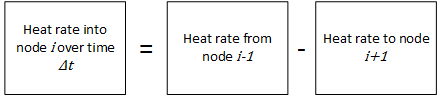
\includegraphics{Figure/thermblocknode1.png}
	\caption{Heat rate balance for conducting nodes}
	\label{fig:thermbalance1}
\end{figure}

Recall that the first node, or the surface node also experiences radiation and convection. The heat rate balance can be easily illustrated by changing the blocks in the previous scheme according to the aforementioned differences. The surface node receives the heat flux, radiates heat away and conducts heat to node $i+1$ (or node 2). No conducted heat is received from node $i-1$ since node 0 does not exist. These changes result in Figure \ref{fig:thermbalance2}.

\begin{figure}[H]
	\centering
	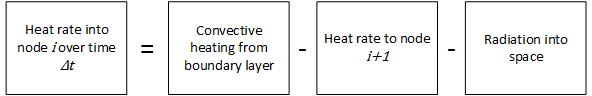
\includegraphics{Figure/thermblocknode2.png}
	\caption{Heat rate balance for conducting nodes}
	\label{fig:thermbalance2}
\end{figure}

Equation \eqref{eq:therm3} can then be altered by adding a $q^n$-term for the convective heating, or heat flux and adding  $\gls{sym:eps}\gls{con:stefanboltzmann}\left(\left(\gls{sym:T}_1^4\right)^n-\left(\gls{sym:T}_\infty^4\right)^n\right)$ to account for the radiation. In here the superscript $n$ stands for timestep $n$. For the last node a similar heat balance can be constructed. Smith says that in this node the radiation and convection terms can omitted since they are much lower than the conductive heat rate in this part \cite{Smith2011}. In this case all heat conducted from node $i-1$ is stored into node $i$ as conduction towards node $i+1$ is not possible.


\subsubsection{Input}
In order to make use of the tool, an input is required. This input consists of thermal conditions and material properties for five different concepts. The thermal properties are the stagnation temperature $ \gls{sym:T0}(t) $ and a stagnation heat flux $ \gls{sym:qdot}_s(t) $. The material properties are the layer thickness $ L_1 $, $ L_2 $, etc., the thermal conductivity $ \gls{sym:k} $, the density $ \gls{sym:rho} $ and lastly the specific heat $ \gls{sym:cp} $.\\

Thermal inputs for the five concepts, temp and flux + graph.\\

Several lay-ups can be analysed, all with a variety of materials. An overview of these materials with their properties is shown in Table  \ref{tab:tpsmatprop}. Where for each material the thermal conductivity, the density, the specific heat, the maximum operative temperature and if applicable, the emissivity are given.

\begin{table}[H]
\caption {TPS Material properties}
\centering
    \begin{tabular}{|l|l|l|l|l|l|}
    \hline
    \textbf{Material}         & \textbf{ $ k $ $ [ \frac{W}{m*K} ] $} & \textbf{ $ \rho $ $ [ \frac{kg}{m^3} ] $} & \textbf{  $ c_{p} $ $ [ \frac{J}{kg*K} ] $ }& \textbf{ $ T_{max} $ $ [ K ] $} &\textbf{ $ \varepsilon $ $ [ - ] $} \\[1.5ex] \hline \hline
     Viton       & 0.202 
& 1842 & 1654 
& 	 & 0.85
 \\ \hline
    Nextel AF14       & 0.150                                                 & 858                                        & 1050                                            & 1373	 & 0.443                                      \\ \hline
    Nextel BF20       & 0.146 
& 1362                                        & 1130 
& 1643	 & 0.443                                      
 \\ \hline
    Nextel XN513      & 0.148                                                 & 1151                                       & 1090                                            & 1673	 & 0.443                                      \\ \hline
    Refrasil C1554-48 & 0.865                                                 & 924                                        & 1172                                            & 1533	 & 0.7                                        \\ \hline
    Refrasil UC100-28 & 0.865                                                 & 890                                        & 1172                                            & 1255  & 0.2                                        \\ \hline
    Hexcel 282 Carbon & 0.5                                                   & 891                                        & 1000                                            & ~ 	 & 0.9                                        \\ \hline
    Pyrogel 6650      & 0.030                                                 & 110                                        & 1046                                            & 923    & ~                                          \\ \hline
    Pyrogel 5401      & 0.0248                                                & 170                                        & 1046                                            & ~  	 & ~                                          \\ \hline
    Refrasil 1800      & 0.085                                                 & 156                                        & 1172                                            & 1255 	 & ~                                          \\ \hline
    Refrasil 2000      & 0.095                                                 & 180                                        & 1172                                            & 1366 	 & ~                                          \\ \hline
    KFA 5             & 0.25                                                  & 98                                         & 1250                                            & 1473* 	 & ~                                          \\ \hline
    Kapton            & 0.12                                                  & 1468                                       & 1022                                            & 673	 & ~                                          \\ \hline
    Upilex            & 0.29                                                  & 1470                                       & 1130                                            & 773 	 & ~                                          \\ \hline
    \end{tabular}
    \label{tab:tpsmatprop}
\end{table}

\subsubsection{Output}
To perform analysis with different material lay-ups certain the tool needs to output the Temperature ($\gls{sym:T}$) at different locations ($\gls{sym:x}$) at different times ($\gls{sym:t}$). This is the result of working out Equation \eqref{eq:therm2} using a correct $\Delta \gls{sym:x}$ and $\Delta \gls{sym:t}$. The output also shows that the results diverge if the stability criterion is not met: $\frac{\gls{sym:alphat}\Delta\gls{sym:t}}{\left(\Delta \gls{sym:x}\right)^2}$ \cite{Holman2002}. Knowing the temperature through the lay-up over time allows to determine the maximum temperature in each layer. Comparing this with maximum allowable temperature, one can check whether a certain lay-up provides enough protection or not.

\subsection{Verification \& Validation}
The full process of verification and validation has shown that the tool does not function correctly. This part is meant to show what the tool does incorrectly and what will be used to continue the verification and validation after the code is debugged.

\subsubsection{Verification}
The verification has been split up in three parts. The first verifies the steady, or time-independent solutions of the tool. The second covers the unsteady, or transient solutions of the tool. The last part verifies the multilayer functionality of the tool.

Although the tool only provides time-dependent results, it is still possible to verify the steady part of the tool. By integrating Fourier's law on heat conduction Equation \eqref{eq:therm4} is formulated. In here $\gls{sym:T}_1$ is the wall temperature and $\gls{sym:T}_2$ the back temperature. The temperature difference should be shown by the tool when it is run for a considerate amount of time with a constant heat flux. It has been shown that for a given constant heat flux the same temperature difference can be seen in the tool from the surface to the back as is calculated with Equation \eqref{eq:therm4}.
\begin{equation}
\frac{q}{\gls{sym:A}} = \frac{\gls{sym:k}}{\Delta \gls{sym:x}}(\gls{sym:T}_1-\gls{sym:T}_2)
\label{eq:therm4}
\end{equation}
For the transient solution one can use the analytical solution (Equation \eqref{eq:therm5}) provided by both Smith and Holman \cite{Smith2011,Holman2012}. Here $\gls{sym:T}_1$ is the wall temperature at $\gls{sym:t}=0$ and $\gls{sym:T}_2$ the back temperature at $\gls{sym:t}=\gls{sym:t}_{end}$. Comparing this solution with the tool shows that the tool does not function correctly. It is not able to give a correct time response, which is essential for the implementation of the tool within the design of the aeroshell.
\begin{equation}
\gls{sym:T}_2-\gls{sym:T}_1 = \frac{2q\sqrt{\gls{sym:alphat}\gls{sym:t}/\pi}}{\gls{sym:k}\gls{sym:A}}\exp\left(\frac{-\gls{sym:x}^2}{4\gls{sym:alphat}\gls{sym:t}}\right)-\frac{q\gls{sym:x}}{\gls{sym:k}\gls{sym:A}}\left(1-erf\frac{\gls{sym:x}}{2\sqrt{\gls{sym:alphat}\gls{sym:t}}}\right)
\label{eq:therm5}
\end{equation}
For the verification of the multilayer Smith suggests to perform an energy balance as energy should be conserved. Looking at Figure \ref{fig:1dthermal} one can see that at any point in time the energy stored in the material lay-up should be the same as the energy convected into the material minus the energy radiated away from the material. \textcolor{red}{SHOW PLOT Energy [J/m2] against time [s]}

\subsubsection{Validation}
In this section the tool is validated against real experimental data. This data has a given applied heat flux and measures temperature throughout the different layers. The tool should show no extreme deviation from the experimental data. \textcolor{red}{GIVE SOURCE...2 cases, rigid and inflatable}


\subsection{Results per concept}
It has not been possible to verify and validate the tool in time due to a bug in the software. Therefore another solution has to be proposed, in order to be able to analyse the different concepts. Note that this method is much more simple than the initial developed tool, and will not be as accurate as the tool. 

\subsubsection{Alternative method}
To compare different concepts it is assumed that the \gls{tps}-mass is dependent on the time integrated total heat rate which gives a heat load. As explained before the incoming heat flux is given at the stagnation point by the aerodynamics group (section \ref{subsec:aerotool}). To obtain this heat flux the aerodynamics group has put different shapes into the same trajectory. For the four inflatable concepts this is a valid trajectory according to the orbit tool. For the rigid concept this is not the case. However, this does not have to be analysed since the structural mass described in section \ref{sec:rigid} already incorporates the \gls{tps}-mass.

In obtaining the incoming heat flux, is assumed that the temperature of the wall is much lower than the stagnation point temperature. The aerodynamics group has calculated stagnation temperatures in the order of tens of thousands Kelvin. Table \ref{tab:tpsmatprop} shows that the commonly used materials for thermal protection in inflatables have a maximum operating temperature of $1700K$. Therefore it is possible to omit the wall temperature in the heat flux as Equation \eqref{eq:stagcoefficient} shows that the resulting heat load shall be a conservative estimate. 

Another consideration made in this method is the radiation as shown in Equation \ref{eq:radiation}. Figure \ref{fig:1dthermal} shows that the incoming heat flux is counteracted by the radiation. Using the Stefan–Boltzmann law the radiation is calculated for different wall temperatures ($\gls{sym:T}_w$) and subtracted from the incoming heat flux to yield the actual heat rate \cite{Holman2002}. This heat rate is then integrated to obtain the heat load. The temperature ($\gls{sym:T}_\infty$) of the space that the wall radiates into is equal to the ambient atmosphere temperature at that point which is given by the astrodynamic tool. It is assumed that the radiation has a constant $\gls{sym:T}_w$, and that the $\gls{sym:T}_w$ does not decrease due to this radiation. In the actual conditions the $\gls{sym:T}_w$ will decrease if the radiation is greater than the incoming heat flux if the entry vehicle for example exits the atmosphere. This indicates that the magnitude of the resulting heat rate, and therefore the heat load, are rough estimates and should only be used to compare the different concepts. Furthermore, the radiation also depends on the emissivity $ \gls{sym:eps}$. This value might change from concept to concept, but it is assumed that all concepts have the same emissivity.

\begin{equation}
\label{eq:radiation}
\gls{sym:qdot}_r = \gls{sym:eps} \cdot \gls{con:stefanboltzmann} \cdot \left( {\gls{sym:T}_w}^4 - {\gls{sym:T}_\infty}^4  \right)
\end{equation}


Since the radiation is strongly dependent on $\gls{sym:T}_w$, the heat load (in $\left[\frac{J}{m^2}\right]$) is calculated using a variable wall temperature. Then the heat load is divided by a reference heat load. This reference heat load is chosen to be the heat load of the stacked toroid. The resulting graph can then be used to compare the concepts.

\subsubsection{Results of the alternative method}
As discussed before, integrating the total heat flux will result in the heat load. the heat loads of the different concepts can be compared as a function of the heat load of the stacked torroid. However, The wall temperature is assumed constant throughout the entire descend. This is not actually the case and therefore a sensitivity analysis is performed. The wall temerature is varied from 500 to 1500 K. The results can be seen in Figure \ref{fig:heatload}.

\begin{figure}[H]
	\centering
	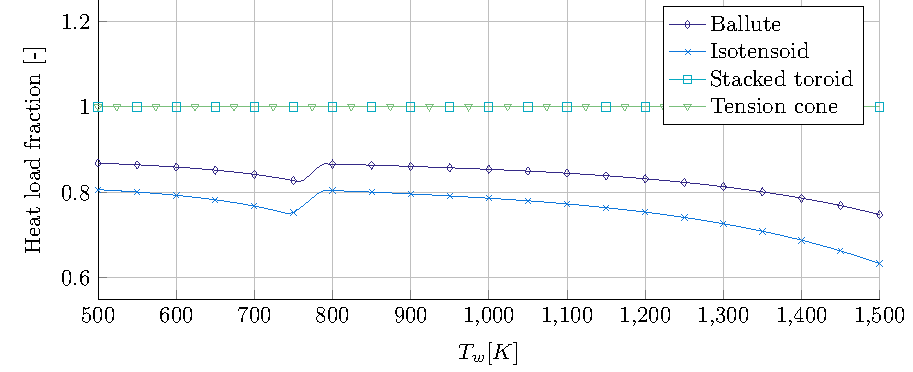
\includegraphics{Figure/heatload.pdf}
	\caption{Standardised heat loads with respect to the isotensoid, varied over different wall temperatures}
	\label{fig:heatload}
\end{figure}

From the figure above, 

\subsection{Conclusion \& recommendations}
The initial approach was to develop a tool to analyse the \gls{tps}-mass for different concepts. Since this tool is not functioning correctly, an alternative analysis method had to be proposed. This approach, described in the previous sections, is very simplistic and resulting values should only be used for comparison of the concepts and not for the actual design of the \gls{tps}.

Since the \gls{tps}-mass of the rigid concept is integrated in the structural mass (section \ref{sec:rigid}), it is not possible to compare the thermal mass of this concept with the inflatable concepts. The inflatable concepts have been compared with the stacked toroid as reference. The tension cone, having the same shape input parameters as input for the aerodynamic tool, receives the same heat load. Therefore it is assumed that the tension cone has the same \gls{tps}-mass as the stacked toroid. The isotensiod is at 79\% and the trailing ballute is at 85\% of the \gls{tps}-mass.

Again it is stressed that the obtained values are rough estimates. Future work should start with the debugging and subsequent verification and validation of the tool. The tool can then be used to design lay-ups that can withstand the incoming heat flux and outgoing radiation and thereby obtain actual values for the \gls{tps}-mass in $\left[\frac{kg}{m^2}\right]$. The tool could also be improved by incorporating the change in thermal conductivity due to the increase in temperature of the materials. Furthermore, the current point of investigation is the stagnation point as the incoming heat flux is the largest at that location. For now the complete heat shield is assumed the be constant in thickness. It can be expected that the required thickness at the edges shall be lower and this could be optimised by using a 3D analysis tool.


Check for material failure other then for thermal reasons.
